\documentclass[12pt,letterpaper]{article}
\usepackage{graphicx,textcomp}
\usepackage{natbib}
\usepackage{setspace}
\usepackage{fullpage}
\usepackage{color}
\usepackage[reqno]{amsmath}
\usepackage{amsthm}
\usepackage{fancyvrb}
\usepackage{amssymb,enumerate}
\usepackage[all]{xy}
\usepackage{endnotes}
\usepackage{lscape}
\newtheorem{com}{Comment}
\usepackage{float}
\usepackage{hyperref}
\newtheorem{lem} {Lemma}
\newtheorem{prop}{Proposition}
\newtheorem{thm}{Theorem}
\newtheorem{defn}{Definition}
\newtheorem{cor}{Corollary}
\newtheorem{obs}{Observation}
\usepackage[compact]{titlesec}
\usepackage{dcolumn}
\usepackage{tikz}
\usetikzlibrary{arrows}
\usepackage{multirow}
\usepackage{xcolor}
\newcolumntype{.}{D{.}{.}{-1}}
\newcolumntype{d}[1]{D{.}{.}{#1}}
\definecolor{light-gray}{gray}{0.65}
\usepackage{url}
\usepackage{listings}
\usepackage{color}

\definecolor{codegreen}{rgb}{0,0.6,0}
\definecolor{codegray}{rgb}{0.5,0.5,0.5}
\definecolor{codepurple}{rgb}{0.58,0,0.82}
\definecolor{backcolour}{rgb}{0.95,0.95,0.92}

\lstdefinestyle{mystyle}{
	backgroundcolor=\color{backcolour},   
	commentstyle=\color{codegreen},
	keywordstyle=\color{magenta},
	numberstyle=\tiny\color{codegray},
	stringstyle=\color{codepurple},
	basicstyle=\footnotesize,
	breakatwhitespace=false,         
	breaklines=true,                 
	captionpos=b,                    
	keepspaces=true,                 
	numbers=left,                    
	numbersep=5pt,                  
	showspaces=false,                
	showstringspaces=false,
	showtabs=false,                  
	tabsize=2
}
\lstset{style=mystyle}
\newcommand{\Sref}[1]{Section~\ref{#1}}
\newtheorem{hyp}{Hypothesis}

\title{Problem Set 1\\
\large Sarah Novotny - 25377750}
\date{Due: October 9, 2025}
\author{Applied Stats/Quant Methods 1}

\begin{document}
	\maketitle
	
	\section*{Instructions}
	\begin{itemize}
	\item Please show your work! You may lose points by simply writing in the answer. If the problem requires you to execute commands in \texttt{R}, please include the code you used to get your answers. Please also include the \texttt{.R} file that contains your code. If you are not sure if work needs to be shown for a particular problem, please ask.
\item Your homework should be submitted electronically on GitHub.
\item This problem set is due before 23:59 on Thursday October 9, 2025. No late assignments will be accepted.
	\end{itemize}
	
	\vspace{1cm}
	\section*{Question 1: Education}

A school counselor was curious about the average of IQ of the students in her school and took a random sample of 25 students' IQ scores. The following is the data set:\\
\vspace{.5cm}

\lstinputlisting[language=R, firstline=44, lastline=44]{PS01_answers_SN.R}  

\vspace{1cm}

\begin{enumerate}
	\item Find a 90\% confidence interval for the average student IQ in the school.\\
	
	\lstinputlisting[language=R, firstline=46, lastline=93]{PS01_answers_SN.R}  
	
	\vspace{.25cm}
	
	\noindent  The 90\% confidence interval for the average student IQ in our sample is:
	\begin{verbatim}
		[94, 104]
		\end{verbatim}
		
		\newpage
	
	\item Next, the school counselor was curious  whether  the average student IQ in her school is higher than the average IQ score (100) among all the schools in the country.\\
	
	\noindent Using the same sample, conduct the appropriate hypothesis test with $\alpha=0.05$.
	\vspace{.25cm}

	\lstinputlisting[language=R, firstline=95, lastline=138]{PS01_answers_SN.R}  
	\vspace{.25cm}
	
	\noindent  A one sided t-test returns a p-value of 0.72  which supports the null hypothesis that the sample mean is less than or equal to 100.  Sad school counselor :( .
	
\end{enumerate}

\newpage

	\section*{Question 2: Political Economy}

\noindent Researchers are curious about what affects the amount of money communities spend on addressing homelessness. The following variables constitute our data set about social welfare expenditures in the USA. \\
\vspace{.5cm}


\begin{tabular}{r|l}
	\texttt{State} &\emph{50 states in US} \\
	\texttt{Y} & \emph{per capita expenditure on shelters/housing assistance in state}\\
	\texttt{X1} &\emph{per capita personal income in state} \\
	\texttt{X2} &  \emph{Number of residents per 100,000 that are "financially insecure" in state}\\
	\texttt{X3} &  \emph{Number of people per thousand residing in urban areas in state} \\
	\texttt{Region} &  \emph{1=Northeast, 2= North Central, 3= South, 4=West} \\
\end{tabular}

\vspace{.5cm}
\noindent Explore the \texttt{expenditure} data set and import data into \texttt{R}.
\vspace{.5cm}

\lstinputlisting[language=R, firstline=142, lastline=150]{PS01_answers_SN.R}  
\vspace{.5cm}
\begin{itemize}

\item
Please plot the relationships among \emph{Y}, \emph{X1}, \emph{X2}, and \emph{X3}? What are the correlations among them (you just need to describe the graph and the relationships among them)?
\vspace{.5cm}

\lstinputlisting[language=R, firstline=153, lastline=196]{PS01_answers_SN.R}  

\vspace{.25cm}

	\begin{figure}[H]\centering
	\caption{\footnotesize relationships among \emph{Y}, \emph{X1}, \emph{X2},  and \emph{X1}.}
	\label{fig:plot_1}
	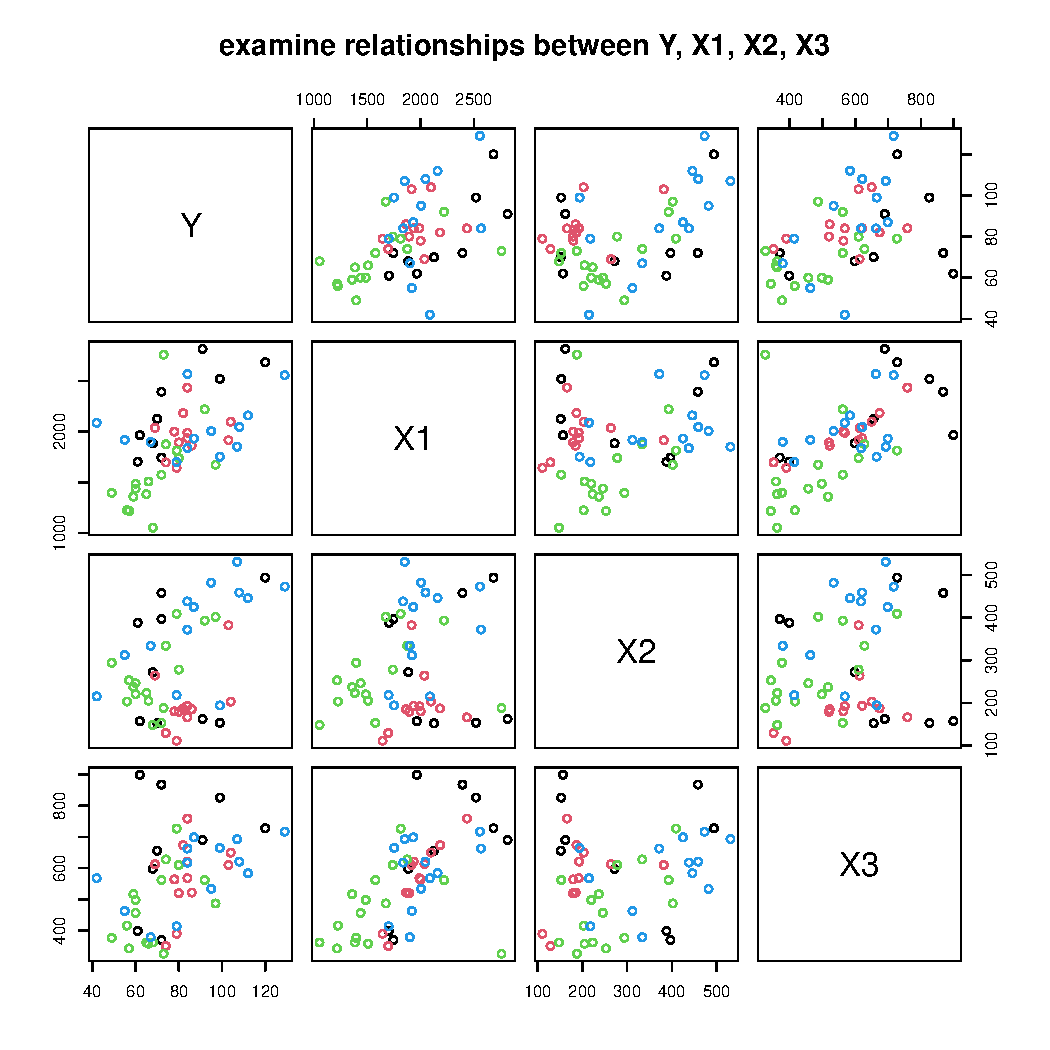
\includegraphics[ width=.75\textwidth]{./Q2_Y_X1_X2_X3.pdf}
	\end{figure}
	
		
% Table created by stargazer v.5.2.3 by Marek Hlavac, Social Policy Institute. E-mail: marek.hlavac at gmail.com
% Date and time: Thu, Oct 09, 2025 - 10:06:30
\begin{table}[H] \centering 
  \caption{} 
  \label{} 
\begin{tabular}{@{\extracolsep{5pt}}lc} 
\\[-1.8ex]\hline 
\hline \\[-1.8ex] 
 & \multicolumn{1}{c}{\textit{Dependent variable:}} \\ 
\cline{2-2} 
\\[-1.8ex] & X3 \\ 
\hline \\[-1.8ex] 
 X1 & 0.216$^{***}$ \\ 
  & (0.042) \\ 
  & \\ 
 Constant & 149.428$^{*}$ \\ 
  & (82.040) \\ 
  & \\ 
\hline \\[-1.8ex] 
Observations & 50 \\ 
R$^{2}$ & 0.354 \\ 
Adjusted R$^{2}$ & 0.341 \\ 
Residual Std. Error & 117.750 (df = 48) \\ 
F Statistic & 26.341$^{***}$ (df = 1; 48) \\ 
\hline 
\hline \\[-1.8ex] 
\textit{Note:}  & \multicolumn{1}{r}{$^{*}$p$<$0.1; $^{**}$p$<$0.05; $^{***}$p$<$0.01} \\ 
\end{tabular} 
\end{table}  

	
		\noindent  In the pairwise compairisons of the variables Y, X1, X2, and X3 in addition to the specific Y vs X1, X2, and X3 also plotted below, there is an simple positive linear correlation with a slope of 0.21  in the graph of X3 vs X1 "Number of people per thousand residing in urban areas in state vs per capita personal income in state".   Though, \emph{Table 1} shows a small R$^{2}$ value leave a large ($>$0.5) unexplained variance.  
		
		\noindent Additionally,  there are  interesting features in the graph of X2 vs X1  "Number of residents per 100,000 that are \emph{financially insecure} in state vs. per capita personal income in state" with two ranges of X2  where X1 varies across the range  of "per capita personal income in the state"

	\begin{figure}[H]\centering
		\caption{\footnotesize relationships between \emph{Y} and \emph{X1}.}
		\label{fig:plot_2}
		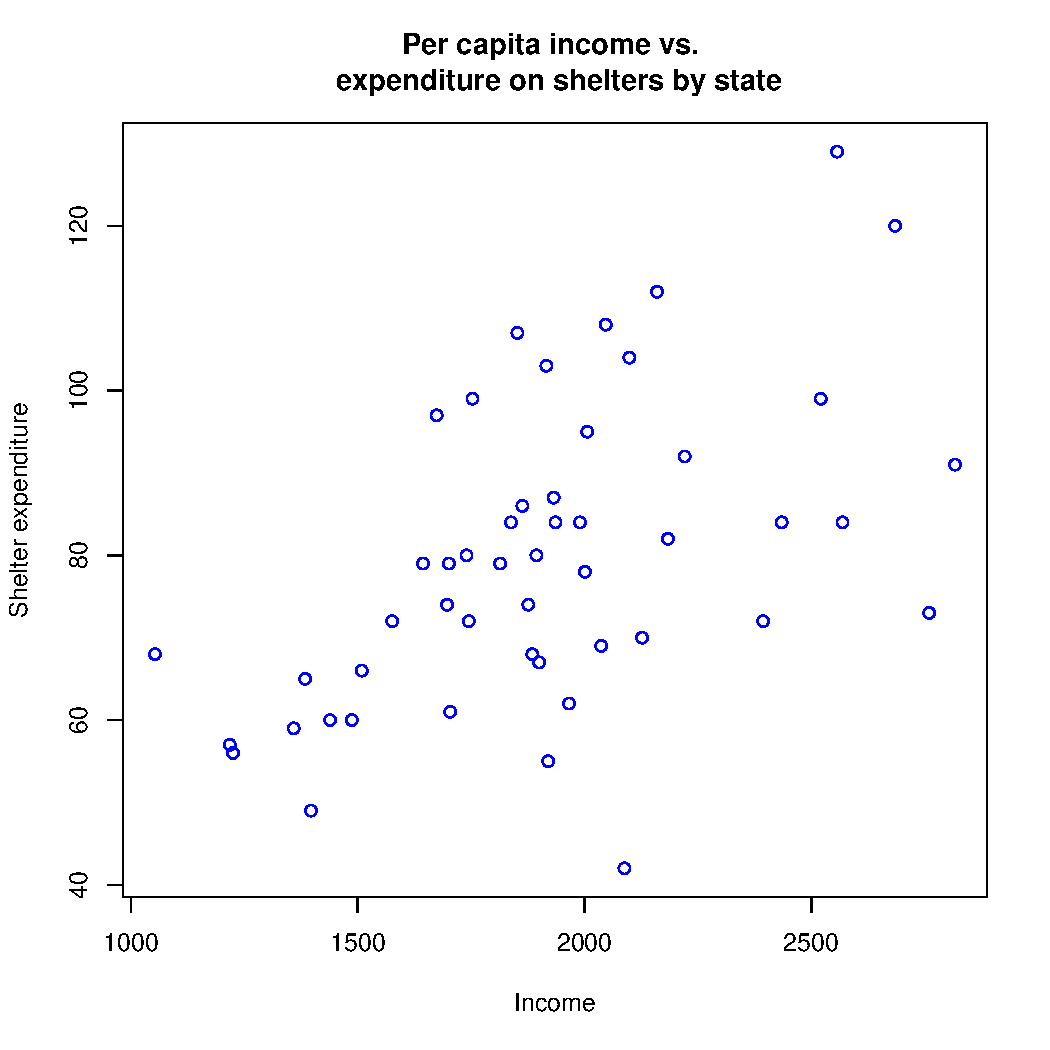
\includegraphics[page=1, width=.75\textwidth]{./Q2_prettier_Y_X1_X2_X3.pdf}
	
	\end{figure}
	
	\noindent  There is a positive correlation between shelter expenditure and per capita income.
	
	\begin{figure}[H]\centering
		\caption{\footnotesize relationships between \emph{Y} and \emph{X2}.}
		\label{fig:plot_3}
	
		\includegraphics[page=2, width=.75\textwidth]{./Q2_prettier_Y_X1_X2_X3.pdf}
	
	\end{figure}
	
		\noindent  There appears to be a u shaped correlation where the shelter expenditure first decreases as the proportion of residents who are insecure increases and then that trend reverses and begins increasing again after the x value of approximately 300/100k .
	
	\begin{figure}[H]\centering
		\caption{\footnotesize relationships between \emph{Y} and \emph{X3}.}
		\label{fig:plot_4}
	
		\includegraphics[page=3, width=.75\textwidth]{./Q2_prettier_Y_X1_X2_X3.pdf}
	\end{figure}
	
		\noindent  There appears to be a linear positive correlation between number of people / one thousand living in urban areas and per capita expenditure on shelters with some strange outliers in very densely populated states.

\item
Please plot the relationship between \emph{Y} and \emph{Region}? On average, which region has the highest per capita expenditure on housing assistance?
\vspace{.5cm}

\lstinputlisting[language=R, firstline=197, lastline=215]{PS01_answers_SN.R}  
\vspace{.25cm}

	\begin{figure}[H]\centering
	\caption{\footnotesize relationships between \emph{Y} and \emph{Region}.}
	\label{fig:plot_5}
	
	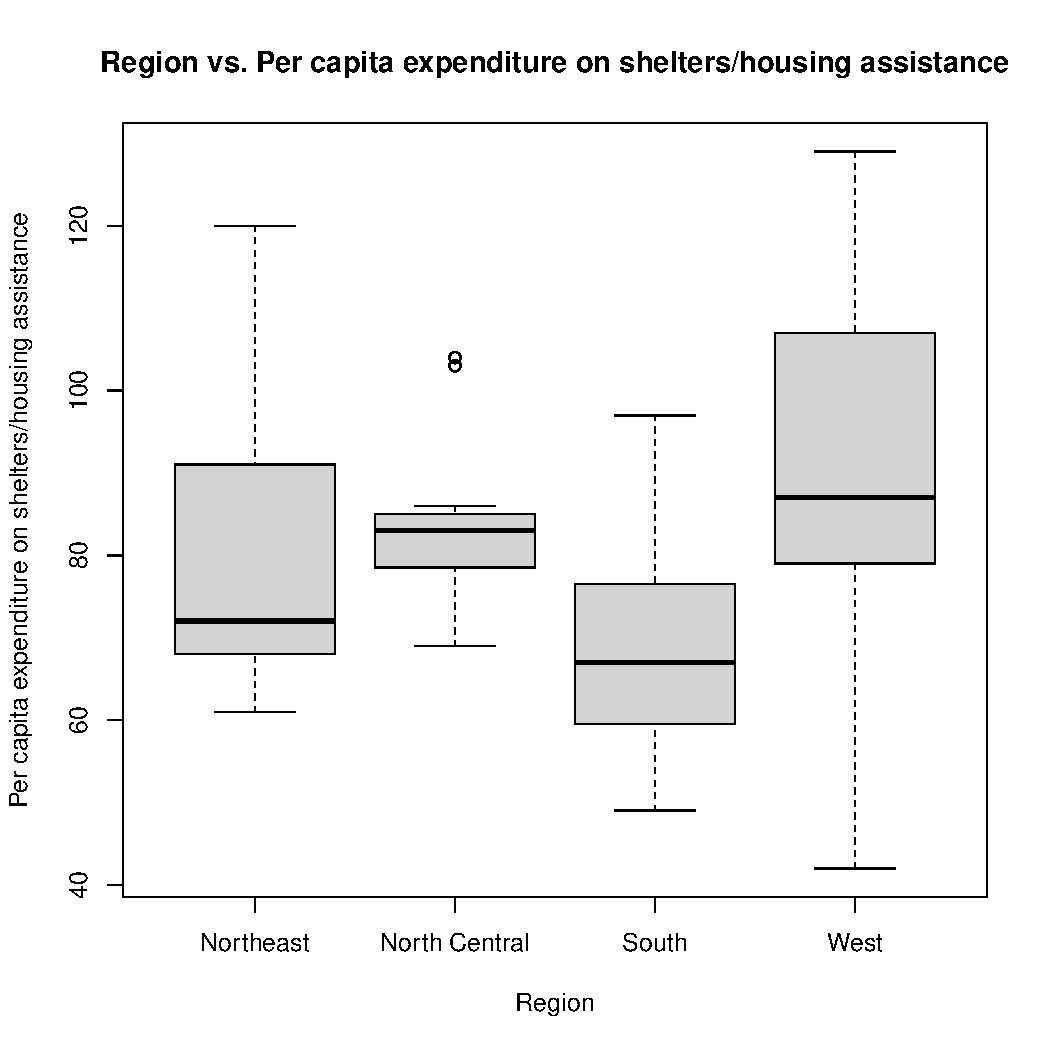
\includegraphics[width=.75\textwidth]{./Q2_average_spending_by_region.pdf}
\end{figure}

	\noindent  On average, the West has the greatest per capita spending on shelter/housing assistance.

\item
Please plot the relationship between \emph{Y} and \emph{X1}? Describe this graph and the relationship. Reproduce the above graph including one more variable \emph{Region} and display different regions with different types of symbols and colors.
\end{itemize}

\lstinputlisting[language=R, firstline=217, lastline=226]{PS01_answers_SN.R}  

	\begin{figure}[H]\centering
	\caption{\footnotesize relationships between \emph{Y} and \emph{X1} with \emph{Region} by color.}
	\label{fig:plot_6}
	
	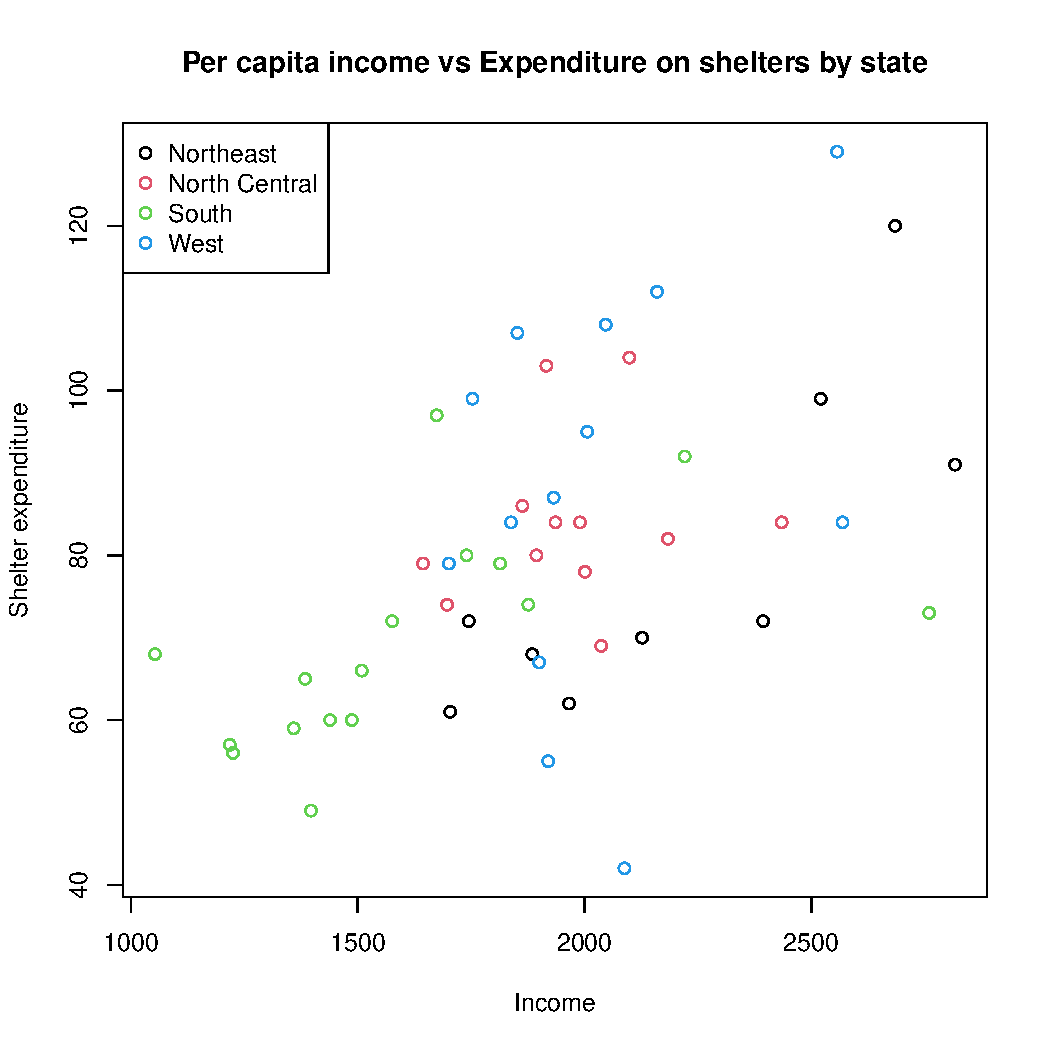
\includegraphics[width=.75\textwidth]{./Q2_scatter_spending_by_region_colored.pdf}
\end{figure}

	\noindent  There is a positive correlation between per capita shelter expenditure and per capita income with large variance and the South region making a particularly poor showing.
	
		\input{./regression_output_X1_Y.tex}
\end{document}
